\section{Realisierung und Implementierung}\label{realisierungundImplementierung}

Diese Kapitel thematisiert die Realisierung und Implementierung. Zunächst wird die Implementierung der SQL-Datenbank vorgestellt, danach folgt die Implementierung des Servers und des Clients. Es werden jeweils ein paar Quellcodeausschnitte näher beleuchtet.

\subsection{Implementierung der SQL Datenbank}

Zuerst wird XAMPP\footnote{https://www.apachefriends.org/de/index.html} heruntergeladen, installiert und eingerichtet. 
\cite{DB5} schreib das XAMPP nur eine lokale Testumgebung simuliert, XAMPP sollte mit der Grundkonfiguration nicht als Webserver im Internet eingesetzt werden, da es Sicherheitslücken aufweist. XAMPP bündelt unterschiedliche freie Software, darunter auch einen lokalen Webserver mit der Datenbank MariaDB und phpMyAdmin.
\\
Im Anschluss wird eine Datenbank für das Projekt mit dem Namen db\_SB\_V1 angelegt.
\\
\\
Anschließend umgesetzt und realisiert werden die entworfenen Tabellen aus dem Kapitel ~\ref{normalisierung}.
Im Zug des Implementierungsprozesses, werden die Tabellen- und Spaltennamen ins Englische übertragen. Folgendes Schema zur Namensgebung wird verwendet.
\begin{itemize}
	\itemsep0pt
	\item Datenbankname: db\_Datenbankname
	\item Tabellenname: tb\_Tabellenname
	\item Spaltenname: cl\_Spaltenname
\end{itemize}
Beispielhaft wird nachfolgend die Tabelle~\ref{3NF Tagesabschluss} implementiert. 



\lstset{language=SQL}
\begin{lstlisting}[frame=htrbl, caption={Erstellung der Tabelle tb\_end of-the-day mit Hilfe des SQL-Behelfes CREATE}, label={lst:tbWaren}]	
CREATE TABLE `tb_end of-the-day` (
	`cl_graduation-date` date NOT NULL,
	`cl_goods-nr` int(10) UNSIGNED NOT NULL,
	`cl_user-nr` int(10) UNSIGNED NOT NULL,
	`cl_graduation-count` int(10) UNSIGNED NOT NULL,
	`cl_graduation-sold` int(10) UNSIGNED NOT NULL,
	`cl_graduation-revenue` decimal(6,2) UNSIGNED NOT NULL
) ENGINE=InnoDB DEFAULT CHARSET=utf8mb4;

\end{lstlisting}	

In Listing~\ref{lst:tbWaren} ist zu sehen wie mithilfe des Befehls CREATE eine neue Tabelle mit den Namen tb\_end of-the-day angelegt wird. 
\\
Folgende Datentypen werden eingesetzt, int (Zahl, von -2.147.483.648 bis 2.147.483.647), VARCHAR (Zeichenkette, bis zu 65.535 Zeichen), decimal (Vorkommastelle Anzahl, Nachkommastelle Anzahl)und DATE (Datum, im Format YYYY-MM-DD).
\\
Durch die Option NOT NULL wird sichergestellt, dass bei Erstellung eines neuen Tupels das Feld einen Wert hat.
Die Option UNSIGNED sorgt dafür, das kein Vorzeichen (+,-) eingeben werden kann, diese hat den Vorteil das nur positive Zeichen eingeben werden können.



\lstset{language=SQL}
\begin{lstlisting}[frame=htrbl, caption={Veränderung der Tabelle tb\_receiptgoods mit Hilfe des SQL-Behelfes ALTER}, label={lst:tbWarenZ}]
ALTER TABLE `tb_end of-the-day`
ADD PRIMARY KEY (`cl_graduation-date`,`cl_goods-nr`),
ADD KEY `cl_goods-nr` (`cl_goods-nr`),
ADD KEY `cl_user-nr` (`cl_user-nr`);


ALTER TABLE `tb_end of-the-day`
ADD CONSTRAINT `tb_end of-the-day_ibfk_1` 
FOREIGN KEY (`cl_goods-nr`) REFERENCES `tb_goods` (`cl_goods-nr`),
ADD CONSTRAINT `tb_end of-the-day_ibfk_2` 
FOREIGN KEY (`cl_user-nr`) REFERENCES `tb_user` (`cl_user-nr`);
			
\end{lstlisting}	


Mit der Anweisung ALTER TABLE können nachträglich unter anderem Optionen hinzugefügt werden, zu sehen ist dieses in Listing \ref{lst:tbWarenZ}. Es wird ein zusammengesetzter Primärschlüssel festgelegt mit der Option ADD PRIMARY KEY, die beiden Spalten cl\_graduation-date und cl\_goods-nr bilden das Schlüsselpaar.
\\
Anschließend wird die Anweisung ALTER TABLE erneut durchgeführt, es wird ein Fremdschlüssel (FOREIGN KEY) für die Spalten cl\_goods-nr und cl\_user-nr generiert. 
In diesem Beispiel, werden die Spalte cl\_goods-nr mit einem Datensatz in der Tabelle tb\_goods, Spalte cl\_goods-nr verknüpft.
\\
\\
\newpage

\begin{figure}[htb]
	\centering
	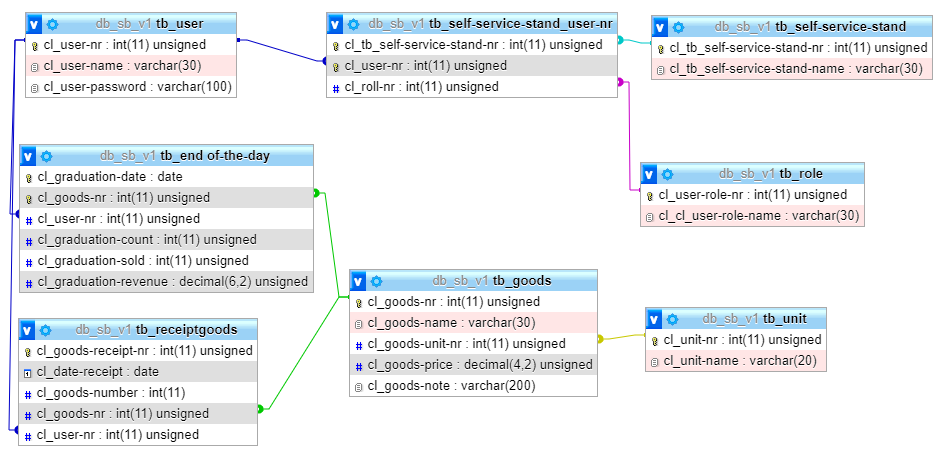
\includegraphics[width=1\textwidth,angle=0]{abb/erstellteTabellen}
	\caption[Übersicht, erstellte Tabellen]{Übersicht, erstellte Tabellen}
	\label{fig:erstellteTabellen}
\end{figure}

Die Abbildung~\ref{fig:erstellteTabellen} stellt die erstellten Tabellen grafisch dar. Aus der Abbildung lassen sich die einzelnen Tabellen, mit den Spalten und den verwendeten Datentypen ablesen. Außerdem können die Primärschlüssel, erkennbar am gelben Schlüssel, leicht identifiziert werden.
Die genutzten Fremdschlüssel lassen sich ebenfalls erkennen, dargestellt durch die farbigen Verbindungslinien.


\subsubsection{MariaDB und phpMyAdmin}\label{MariaDB und phpMyAdmin}
MariaDB ist ein bekanntestes Datenbankmanagementsystem (DBMS), dieses wird in diesem Projekt genutzt. In diesem Kapitel wird erläutert, warum dieses System verwendet wird.
\\

MariaDB\footnote{https://mariadb.com} wurde im Jahr 2009 veröffentlicht. Das DBMS unterliegt einer GPL2 Open-Source Lizenz, das heißt sowohl private als auch kommerzielle Nutzung ist erlaubt. Entwickelt wurde MariaDB von Michael Widenius, er entwickelte ebenfalls MySQL, aus diesem Grund gibt es sehr viele Gemeinsamkeiten. 
\\
MariaDB hat eine gute Geschwindigkeit und Performance, bei der Durchführung von Datenbankabfragen. Die Seite \cite{DB4} schreibt \grqq Features wie Hochverfügbarkeit, Security, Interoperabilität und Performanceverbesserungen aufweist.\grqq{} bietet MariaDB. 
\\
Damit die Verwaltung der Datenbank komfortabler ist, wird die Software phpMyAdmin\footnote{https://www.phpmyadmin.net} verwendet. PhpMyAdmin ist weitverbreitet und die Standartsoftware zum Verwalten von Datenbanken. 

\subsection{Implementierung des Spring Boot Servers}

Für die Entwicklung des Servers wurde Spring Boot gewählt. Spring Boot ist eine Open Source Software und kann kostenlos genutzt werden. Außerdem existiert eine große Community, die bei Fragen weiterhelfen kann. Spring Boot bietet außerdem einen großen Funktionsumfang. Es lassen sich leicht neue Funktionen usw. integrieren. Allerdings erfordert Spring Boot etwas Einarbeitungszeit.
 \\
 \\
Nachfolgend werden einige Quellcodeausschnitte etwas genauer erläutert. Der komplette Quellcode der Klasse ist im Anhang \ref{QuellcodeServer} zu finden.
Zuerst werden zwei Klassen aus dem Paket model dargestellt, anschließend werden aus den Paketen controller, service und repoitory ebenfalls Klassen vorgestellt. 
\\
\\
Um die objektrelationale Abbildung der Datenbank zu erleichtern, wird JPA(Java Persistence API) verwendet, JPA ist im Spring Boot Framework enthalten. \cite{JPA} schreibt \grqq Die Java Persistence API (JPA) des Java Community Process ist ein Standard für das Objekt-relationale Mapping (ORM) von Java-Objekten. ORM ist ein Verfahren zur Speicherung von Objekten in Datenbanken - Klassen und Objekte werden auf Tabellen und Zeilen abgebildet.\grqq{}. 

\subsubsection{Beispielcodeausschnitte aus Model-Klassen}

Die Klasse EndOfTheDay \ref{lst:EndOfTheDay} befindet sich im Paket model, die Klasse bildet die Datenbankstruktur der Tabelle tb\_end of\_the\_day ab. Die Datenbanktabelle enthält unter anderem einen zusammengesetzten Primärschlüssel, sowie drei Fremdschlüssel. 
\\
\lstset{language=java}
\begin{lstlisting}[frame=tb, caption={Das Listing zeigt einen Ausschnitt aus der Klasse EndOfTheDay}, label={lst:EndOfTheDayAus}]
@Table(name = "tb_end of_the_day", indexes = {
	@Index(name = "cl_user_nr", columnList = "cl_user_nr"),
	@Index(name = "cl_goods_nr", columnList = "cl_goods_nr"),
	@Index(name = "cl_self_service_stand_nr", columnList = "cl_self_service_stand_nr")
})
@Setter
@Getter
@Entity
public class EndOfTheDay {
	
	/**
	* ID End of the Day.
	*/
	@EmbeddedId
	private EndOfTheDayId id;
	
	/**
	* Refers to a user ID.
	*/
	@ManyToOne
	@JoinColumn(name = "cl_user_nr", nullable = false)
	private User userNr;
\end{lstlisting}

Im Codeausschnitt \ref{lst:EndOfTheDayAus} Zeile 1, ist die Zuordnung einer bereits bestehenden Tabelle in einer Datenbank mithilfe der JPA-Annotationen @Table zu sehen. Anschließend wird in den Zeilen 2 bis 5 die Fremdschlüsselverknüpfung durchgeführt, dabei wird auf eine Spalte in einer anderen Tabelle verwiesen.
\\
\\
Die Annotationen @Setter und @Getter in Zeile 6 und 7 sorgen dafür, das die Getter und Setter Methoden nicht mehr implementiert werden müssen. Sondern mithilfe des Java-Framework Lombok automatisch intrigiert werden.
\\
\\
Die JPA-Annotationen @Entity in der 8 Zeile bewirkt das automatisch alle Attribute in der Klasse auf gleichnamige Datenbankspalten (Mapping) abgebildet werden. Es kann der Fall auftreten, dass die Attribute und Spaltennamen unterschiedlich heißen, wie z. B. in Zeile 22 Mit der Annotation @JoinColumn(name = \grqq{}cl\_user\_nr\grqq{}) in Zeile 21 wird der Tabellenspaltname zugewiesen.
\\
\\
Da es sich bei dem Attribute User um eine Fremdschlüsselverknüpfung handelt, wird in Zeile 20 eine 1:n Beziehung hinzugefügt, es wird ein User-Objekt deklariert.
\\
\\
Bei der ID handelt es sich um einen zusammengesetzten Primärschlüssel, siehe Zeile 13 und 19. Es wird ein EndOfTheDayId-Objekt erstellt. Im Listing \ref{lst:EndOfTheDayIdAus} ein Codeausschnitt der Klasse EndOfTheDayId abgebildet. In Zeile 8 und 14 sind die Attribute zu sehen aus denen sich der zusammengesetzte Primärschlüssel definiert. Die Annotationen in Zeile 1 deutet darauf hin, dass in dieser Klasse ein zusammengesetzter Primärschlüssel vorhanden ist.
\\
\lstset{language=java}
\begin{lstlisting}[frame=tb, caption={Das Listing zeigt einen Ausschnitt aus der Klasse EndOfTheDayId}, label={lst:EndOfTheDayIdAus}]
@Embeddable
public class EndOfTheDayId implements Serializable {
	
	/**
	* serialVersionUID
	*/
	private static final long serialVersionUID = 4548732131340178144L;
	
	/**
	* End of the day date.
	*/
	@Column(name = "cl_graduation_date", nullable = false)
	private LocalDate graduationDate;
	
	/**
	* The commodity number.
	*/
	@Column(name = "cl_goods_nr", nullable = false)
	private Integer goodsNr;
\end{lstlisting}

\subsubsection{Beispielcodeausschnitte aus Repository-Interfaces}

Im Paket repository sind Interfaces enthalten, die für Datenbankoperationen zuständig sind. Es handelt sich nicht um Standard JPA, sondern es wird Spring Data JPA verwendet. Genutzt wird die Kurzschreibweise für Abfragen.

\lstset{language=java}
\begin{lstlisting}[frame=tb, caption={Das Listing zeigt einen Ausschnitt aus dem Interface GoodsNameRepository}, label={lst:GoodsNameRepositoryAus}]
@Repository
public interface GoodsNameRepository extends JpaRepository<GoodsName, Integer> {
	
	//Query list of all goods names, sorted by unit name.
	List<GoodsName> findByOrderByGoodsNameAsc();
	
	//Query, goods name with the name exists.
	boolean existsByGoodsNameIs(String goodsName);
	
}
\end{lstlisting}

Im Listing \ref{lst:GoodsNameRepositoryAus} ist das Repository des Interfaces GoodsNameRepository abbildet. Das Interface erbt vom Interface JpaRepository Zeile 2. \\
In der Zeile 5 ist eine Datenbankabfrage zu sehen die eine sortierte Liste mit allen vorhanden Einträgen in der Tabelle zurückliefert. 
\\
Eine weitere Abfrage ist in Zeile 8, diese Abfrage liefert ein True zurück, sobald ein Eintrag mit der eingebenden Zeichenkette übereinstimmt. 
\\
\lstset{language=java}
\begin{lstlisting}[frame=tb, caption={Das Listing zeigt einen Ausschnitt aus dem Interface ReceiptGoodRepository}, label={lst:ReceiptGoodRepositoryAus}]
List<ReceiptGoods> findByDateReceiptAndGoodsNr_GoodsId(LocalDate dateReceipt, Integer goodsId);
\end{lstlisting}

Das Listing \ref{lst:ReceiptGoodRepositoryAus} liefert ein Beispiel für eine Verknüpfte Und-Abfrage. Außerdem wird in der Tabelle nach einem Fremdschlüsseltribut (GoodsNr\_GoodsId) gesucht.

\subsubsection{Beispielcodeausschnitte aus einer Controller-Klasse}


\lstset{language=java}
\begin{lstlisting}[frame=tb, caption={Das Listing zeigt einen Ausschnitt aus der Klasse unitController}, label={lst:unitControllerAus}]
@RestController
@RequestMapping("/unit")
public class UnitController {
		
	/**
	* unitRepository to handle unit information.
	*/
	private final UnitRepository unitRepository;
	
	/**
	* goodsRepository to handle goods information.
	*/
	private final GoodsRepository goodsRepository;
	
	/**
	* Service to handle self-service stand information logic.
	*/
	private final UnitService unitService;
	
	public UnitController(UnitRepository unitRepository, GoodsRepository goodsRepository, UnitService unitService) {
		this.unitRepository = unitRepository;
		this.goodsRepository = goodsRepository;
		this.unitService = unitService;
	}
\end{lstlisting}

In Zeile 1 wird festgelegt, dass es sich bei der Klasse um einen Rest-Controller handelt. 
\\
Mapping wird in der 2. Zeile durchgeführt.\cite{mapping} beschreibt, das es beim Mapping \glqq um die Konversion von zwei verschiedenen Adressräumen.\glqq{} geht.\glqq Dabei werden die Daten eines Adressraums auf einen zweiten Adressraum abgebildet.\glqq{}
\\
Alle Klassen mit der Annotation @Repository, @Controller, @Service oder @Component werden automatisch als Bean erkannt und registriert. In der Spring Dokumentation \cite{spring} steht das ein Bean, ein Objekt ist, das von einem Spring IoC-Container instanziiert, assembliert und verwaltet wird.
\\
\\
Es wird das Endwurstmuster Dependency Injektion verwendet. Dieses besagt, das Komponenten und Klassen soweit möglich unabhängig von anderen Klassen sein sollen, bekannt auch als lose Kopplung, erklärt \cite{Dependency}.  \grqq Als Dependency Injection bezeichnet man in der objektorientierten Programmierung eine externe Instanz, die die Abhängigkeiten von Objekten im Vorhinein regelt \grqq{} \cite{Spring1}.
\\
In diesem Projekt wird mithilfe von Constructor-Injection (Konstruktor-Injektion) das Objekt injiziert. Dieses ist in den Zeilen 8 bis 24 zu erkennen, es werden sowohl Repositoryklassen und eine Serviceklasse eingebunden, Zeilen 8 bis 18. Diese werden im Konstruktor injizierten, Zeile 20 bis 24.
\\
\lstset{language=java}
\begin{lstlisting}[frame=tb, caption={Das Listing zeigt eine Methode aus der Klasse unitController}, label={lst:unitControllerAusM}]
/**
* Method returns a sorted list with all units.
*
* @return json list with all units
*/
@GetMapping(path = "/", produces = MediaType.APPLICATION_JSON_VALUE)
    private ResponseEntity<List<Unit>> getUnits() {
	
	//Return sorted list, sorted by unit name.
	return new ResponseEntity<>(unitService.getUnitsList(), HttpStatus.OK);
}
\end{lstlisting}

Im Listing \ref{lst:unitControllerAusM} ist eine Methode aus der Klasse UnitController abgebildet. Diese Methode wird durch die REST-Schnittstelle GET /unit angesprochen (\ref{lst:unitControllerAus}). Der Pfad /unit wurde bereits am Klassenanfang festgelegt \ref{lst:unitControllerAus} Zeile 1. Da in dieser Klasse nur eine Get-Schnittstelle angesprochen wird, kann diese eindeutig infiziert werden, eine weitere Pfad Angabe ist nicht nötig. 
\\
Die Methode gibt eine Json-Liste und einen HttpStatus zurück. Diese ist in Zeile 10 implementiert. Außerdem ist zu sehen, wie eine Service Bean aufgerufen wird, (unitService.getUnitsList()). Dadurch wird die entsprechende Methode in der Serviceklasse ausgelöst.














\subsection{Implementierung des Angular-Clients}

Diese Kapitel erläuterte die Implementierung des Angular-Clients. Zuerst wird auf die Implementierung der grafischen Benutzeroberfläche eingegangen. Danach folgt die Implementierung des Hintergrundbereiches.


\subsubsection{Implementierung der grafischen Benutzeroberfläche (Frontend)}

In diesem Kapitel wird auf die Implementierung der grafischen Benutzeroberfläche eingegangen, nachfolgend werden einige Quellcodeausschnitte gezeigt. Zuerst wird kurz auf das Grid Layout eingegangen.
\\
\\
\newpage
Eines der Hauptmerkmale von Angular ist, das dieses komponentenbasiert arbeitet. 
Da bereits bei der Konzeption die Oberflächen in Komponenten eingeteilt worden sind, bietet es sich an, Angular zu verwenden.
\\
\\
Jede dieser Komponenten enthält eine CSS-Datei, HTML-Datei und eine Typscript-Datei. In diesem Kapitel wird auf die CSS-Datei und HTML-Datei eingegangen.
\\
\\
Das Gestaltungsraster wird mithilfe CSS Grid Layout gestaltet. Mithilfe von Grid lässt sich eine Seite in einzelne Raster aufteilen, die Flächen müssen nicht die gleiche Größe haben, sondern nur rechteckig sein. 
Die Komponenten werden den Rasterzellen zugewiesen.

\lstset{language=html}
\begin{lstlisting}[frame=tb, caption={Umsetzung des Grid-Layout}, label={lst:grid}]
.container {
	display: grid;
	grid-template-columns: 0.5fr 2fr 8fr 2fr 0.5fr;
	grid-template-rows: 0.4fr 3.4fr 0.4fr 0.4fr;
	gap: 0px 0px;
	grid-auto-flow: row;
	grid-template-areas:
	"navbar navbar navbar navbar navbar"
	"main main main main main"
	"selectSelf selectSelf . . ."
	"footer footer footer footer footer";
}

.navbar {
	grid-area: navbar;
	background: var(--colorGray);
}
	\end{lstlisting}


Im Listing~\ref{lst:grid} ist ein Ausschnitt aus einer CSS-Datei zusehen. In dieser, wird die Vorlage aus dem Kapitel 4 Entwurf der grafischen Benutzeroberfläche ~\ref{fig:Hauptmenü} mit Grid umgesetzt.
\\
In den Zeilen 3 und 4 ist zu sehen, wie Größe und Anzahl der Spalten und Zeilen festgelegt wird, es gibt fünf Spalten und vier Zeilen. In Zeile 7 bis 11 werden den Rasterbereichen Namen zugewiesen, der Bereich navbar (Hauptmenü) ist beispielsweise in Zeile eines, Spalte zwei bis vier zu finden.
 \\
Die Zeilen 14 bis 17 zeigen, wie einer CSS-Klasse der Grid-Bereich navbar zugewiesen wird. In Zeile 16 wird die Farbe des Hintergrundbereiches festgelegt, die Farbe ist in einer Variabel gespeichert. Dieses hat den Vorteil, dass die festgelegt Farbe schnell und leicht änderbar ist.
\\


\lstset{language=html}
\begin{lstlisting}[frame=tb, caption={Zuweisung der Komponenten in HTML}, label={lst:html}]
<div class="container">
	<div class="navbar">
		<app-navbar></app-navbar>
	</div>
	<div class="main">
		<router-outlet></router-outlet>
	</div>
	<div class="footer">
		<app-footer></app-footer>
	</div>
\end{lstlisting}

Im Listing~\ref{lst:grid} ist ein Teilausschnitt einer HTML-Datei abgebildet.
Das Listing~\ref{lst:html} veranschaulicht die Zuweisung der CSS-Klassen z. B. in Zeile 2.
\\
Außerdem ist zu sehen wie erstellte Angular-Komponenten eingebunden werden, Zeile 3 und 9.
\\
In Zeile 6 wird das Router-Outlet im Hauptbereich implementiert. Angular sorgt automatisch dafür dass die richtige Komponente eingefügt wird. Mithilfe von vordefinierten internen Routinezuweisungen wird die passende Komponente ausgewählt. Mehr dazu im nachfolgenden Kapitel.
\\

\lstset{language=html}
\begin{lstlisting}[frame=tb, caption={Schleifen und Abfragen in HTML}, label={lst:html1}]
<tr (click)="setValues(goods.goodsId)" *ngFor="let goods of searchResultList">
	<td>{{goods.goodsId}}</td>
	<td>{{goods.goodsName}}</td>
	<td>{{goods.unitName}}</td>
	<td>{{goods.goodsPrice}}</td>
	<td>{{goods.goodsNote}}</td>
	<div *ngIf=goods.goodsActive>
		<td>Ja</td>
	</div>
	<div *ngIf=!goods.goodsActive>
		<td>Nein</td>
	</div>
</tr>
\end{lstlisting}

Im Listing~\ref{lst:html1} ist eine forEach-Schleife und zwei IF-Abfragen zu sehen. 
Die forEach-Schleife befindet sich in der Zeile 1,(*ngFor=\grqq{}let goods of searchResultList) es wird eine Liste (searchResultList), diese wurde in der dazugehörigen TypeScript-Datei initialisiert, durchlaufen. Der nachfolgende HTML-Code wird dabei so oft ausgeführt wie es der Länge der Liste entspricht. Für jeden Schleifendurchlauf wird ein Element in die Variabel goods gespeichert. Diese wird nachfolgende ausgeben. 
\\
In Zeile 7 wird eine If-Abfrage durchgeführt, dabei wird überprüft, ob goods.goodsActive mit dem Wert True initialisiert worden ist. Ist dieses der Fall werden alle Elemente im nachfolgenden Div-Element ausgeführt.

\subsubsection{Implementierung des Hintergrundbereichs (Backend)}

Es werden in diesem Kapitel einige TypeScript-Quellcodeausschnitte gezeigt.

\lstset{language=java}
\begin{lstlisting}[frame=tb, caption={Festlegung der internen Routen in Angular}, label={lst:html2}]
const myRoutes: Routes = [
{
	path: '',
	component: MainScreenComponent,
	children: [
	{
		path: 'goods',
		component: GoodsComponent,
		children: [
		{
			path: 'overview',
			component: OverviewGoodsComponent
		},
		{
			path: 'new',
			component: NewGoodsComponent
		},
		{
			path: 'change',
			component: ChangeGoodsComponent
		}, {
			path: 'settings',
			component: SettingsGoodsComponent
		}
		]
	},	
\end{lstlisting}

Im ersten Listing~\ref{lst:html2} dieses Kapitels ist zu sehen, wie die internen Routen in der Konstante myRoutes gespeichert werden, Zeile 1. Mithilfe von internen Routen ist es möglich innerhalb von Angular zu navigieren oder die Ansichten zu ändern. Dieses wird im Quellcode Listing \ref{lst:html1} Zeile 6 genutzt. 
\\
Im Listing \ref{lst:html3} ist HTML-Code abgebildet, in der Zeile 4 ist ein interner Link zu sehen, dieser leitet weiter zum Pfad /goods/overview. Es können Eltern-Pfad-Routen und deren Kinderelemente festgelegt werden, dargestellt im Listing~\ref{lst:html2} Zeile 5 bis 26.
\\
Dass RouterModule welches importiert wird, übernimmt das Routing für den Entwickler.

\lstset{language=java}
\begin{lstlisting}[frame=tb, caption={Festlegung der internen Routen in Angular}, label={lst:html3}]

<div class="btn btn-default link-menu">
	<i class="fa fa-id-card-o"></i> 
	<a routerLink="/goods/overview">Waren</a>
</div>
	\end{lstlisting}

Folgender Quellcode sogt dafür, dass eine Get-Anfrage an den Server gesendet wird.

\lstset{language=java}
\begin{lstlisting}[frame=tb, caption={Get-Anfrage an den Server}, label={lst:html4}]
	
  private loadGoods() {
	
	//set url
	let url = 'goods/' + localStorage.getItem('key_selfServiceStand_name');
	
	//communication Server
	this.communication
	.serverCommunication(url, '', 'get', true)
	.subscribe((response: any) => {
		
		//save entry in list
		for (var entry of response) {
			this.goodsList.push({
				goodsId: entry.goodsId,
				goodsName: entry.goodsNameNr.goodsName,
				unitName: entry.goodsUnitNr.unitName,
				goodsPrice: entry.goodsPrice,
				goodsNote: entry.goodsNote,
			});
		}
		
	}, error => {
		console.log(error);
	}
	);
}
\end{lstlisting}

Im Listing~\ref{lst:html4} ist zu sehen wie eine Anfrage an den Server gesendet wird, es wird eine Liste mit allen verfügbaren Waren angefordert. Zuerst wird ein Teil der URL in der Variabel url gespeichert. Anschließend wird eine Verbindung zum Server aufgebaut (Zeile 8 bis 10), die restlichen erforderlichen Informationen sind in der Service Klasse server-communication.service hinterlegt, unter anderem der Token, URL usw.. 
\\
\\
\\
Bei erfolgreicher Übermittlung werden die anforderten Daten in der mehrdimensionalen Liste goodsList gespeichert (Zeilen 13 bis 21). Ansonsten wird eine Fehlermeldung ausgeben (Zeile 24). 